%!TEX root = ../rapport.tex
%!TEX encoding = UTF-8 Unicode

% Chapitres "Introduction"

% modifié par Francis Valois, Université Laval
% 31/01/2011 - version 1.0 - Création du document

\chapter{Schémas électroniques 2$^{e}$ itération}
\label{electronics}
Le modèle de microcontrôleur employé est un Stellaris LM3S9B92. Les différentes entrées et sorties ont été fixées sur un circuit imprimé (PCB) dont le schéma est présenté à la figure \ref{fig:plan_micro}. 
\paragraph{}L'ensemble des circuits électriques est placé devant des circuits de fusibles dont le schéma est présenté à la figure \ref{fig:protection}. Cela a pour but d'éviter une surcharge de courant dans la branche. Par ailleurs, ces circuits sont actionnables par des interrupteurs placés devant les circuits respectifs. 
\paragraph{}L'alimentation 5V des périphériques est réalisée au moyen d'un circuit Buck 5V, le schéma est présenté à la figure \ref{fig:alim5V}.
\paragraph{}Laimentation 24V du préhenseur et du Mac mini est réalisée au moyen d'un circuit Boost acheté chez un détaillant, pour lequel on ne dispose pas du circuit. La tension de sortie est variable avec un potentiomètre. La tension d'entrée est directement celle de la batterie. Une photo du dispositif est disponible à la figure \ref{fig:alim24Vphoto}.
\paragraph{}Le circuit de démodulation du signal Manchester présent sur les tables est réalisé au moyen du circuit présenté à la figure \ref{fig:manchester}. La clef de ce circuit est le LM567 qui est un circuit intégré permettant de syntoniser le signal d'antenne selon une largeur de bande que l'on établit au moyen des capacités présentes sur les différentes branches. Le LM567 permet d'isoler directement l'enveloppe du signal. Un comparateur à hystérésis est placé à la sortie du LM567 de manière à rendre plus uniformes et abruptes les transitions dans le signal d'enveloppe. 
\paragraph{}Le circuit de commande du préhenseur est présenté à la figure \ref{fig:prehenseur}. Il n'est composé que d'un transistor Mosfet qui permet d'activer la conduction du préhenseur (avec un courant proche de 150mA), directement à partir du microcontrôleur. Une diode de roue libre permet de décharger l'énergie de la bobine (préhenseur) lors des transitions.
\paragraph{}Le circuit de commande de la DEL est présenté à la figure \ref{fig:del_verte}. Il n'est composé que d'un transistor Mosfet qui permet d'activer la conduction de la DEL, une résistance de 100$\Omega$ permet de limiter le courant dans la DEL.

\begin{figure}
\centering
\includegraphics[scale=0.5]{fig/plan_micro.jpg}
\caption{Figure présentant les plans de l'alimentation 5V pour les périphériques}
\label{fig:plan_micro}
\end{figure}

\begin{figure}
\centering
\includegraphics[scale=0.5]{fig/plan_circuit_protection.png}
\caption{Figure présentant le circuit de protection des circuits électriques}
\label{fig:protection}
\end{figure}

\begin{figure}[htbp]
\centering
\includegraphics[scale=0.5]{fig/alim_5V.png}
\caption{Figure présentant les plans de l'alimentation 5V pour les périphériques}
\label{fig:alim5V}
\end{figure}

\begin{figure}[htbp]
\centering
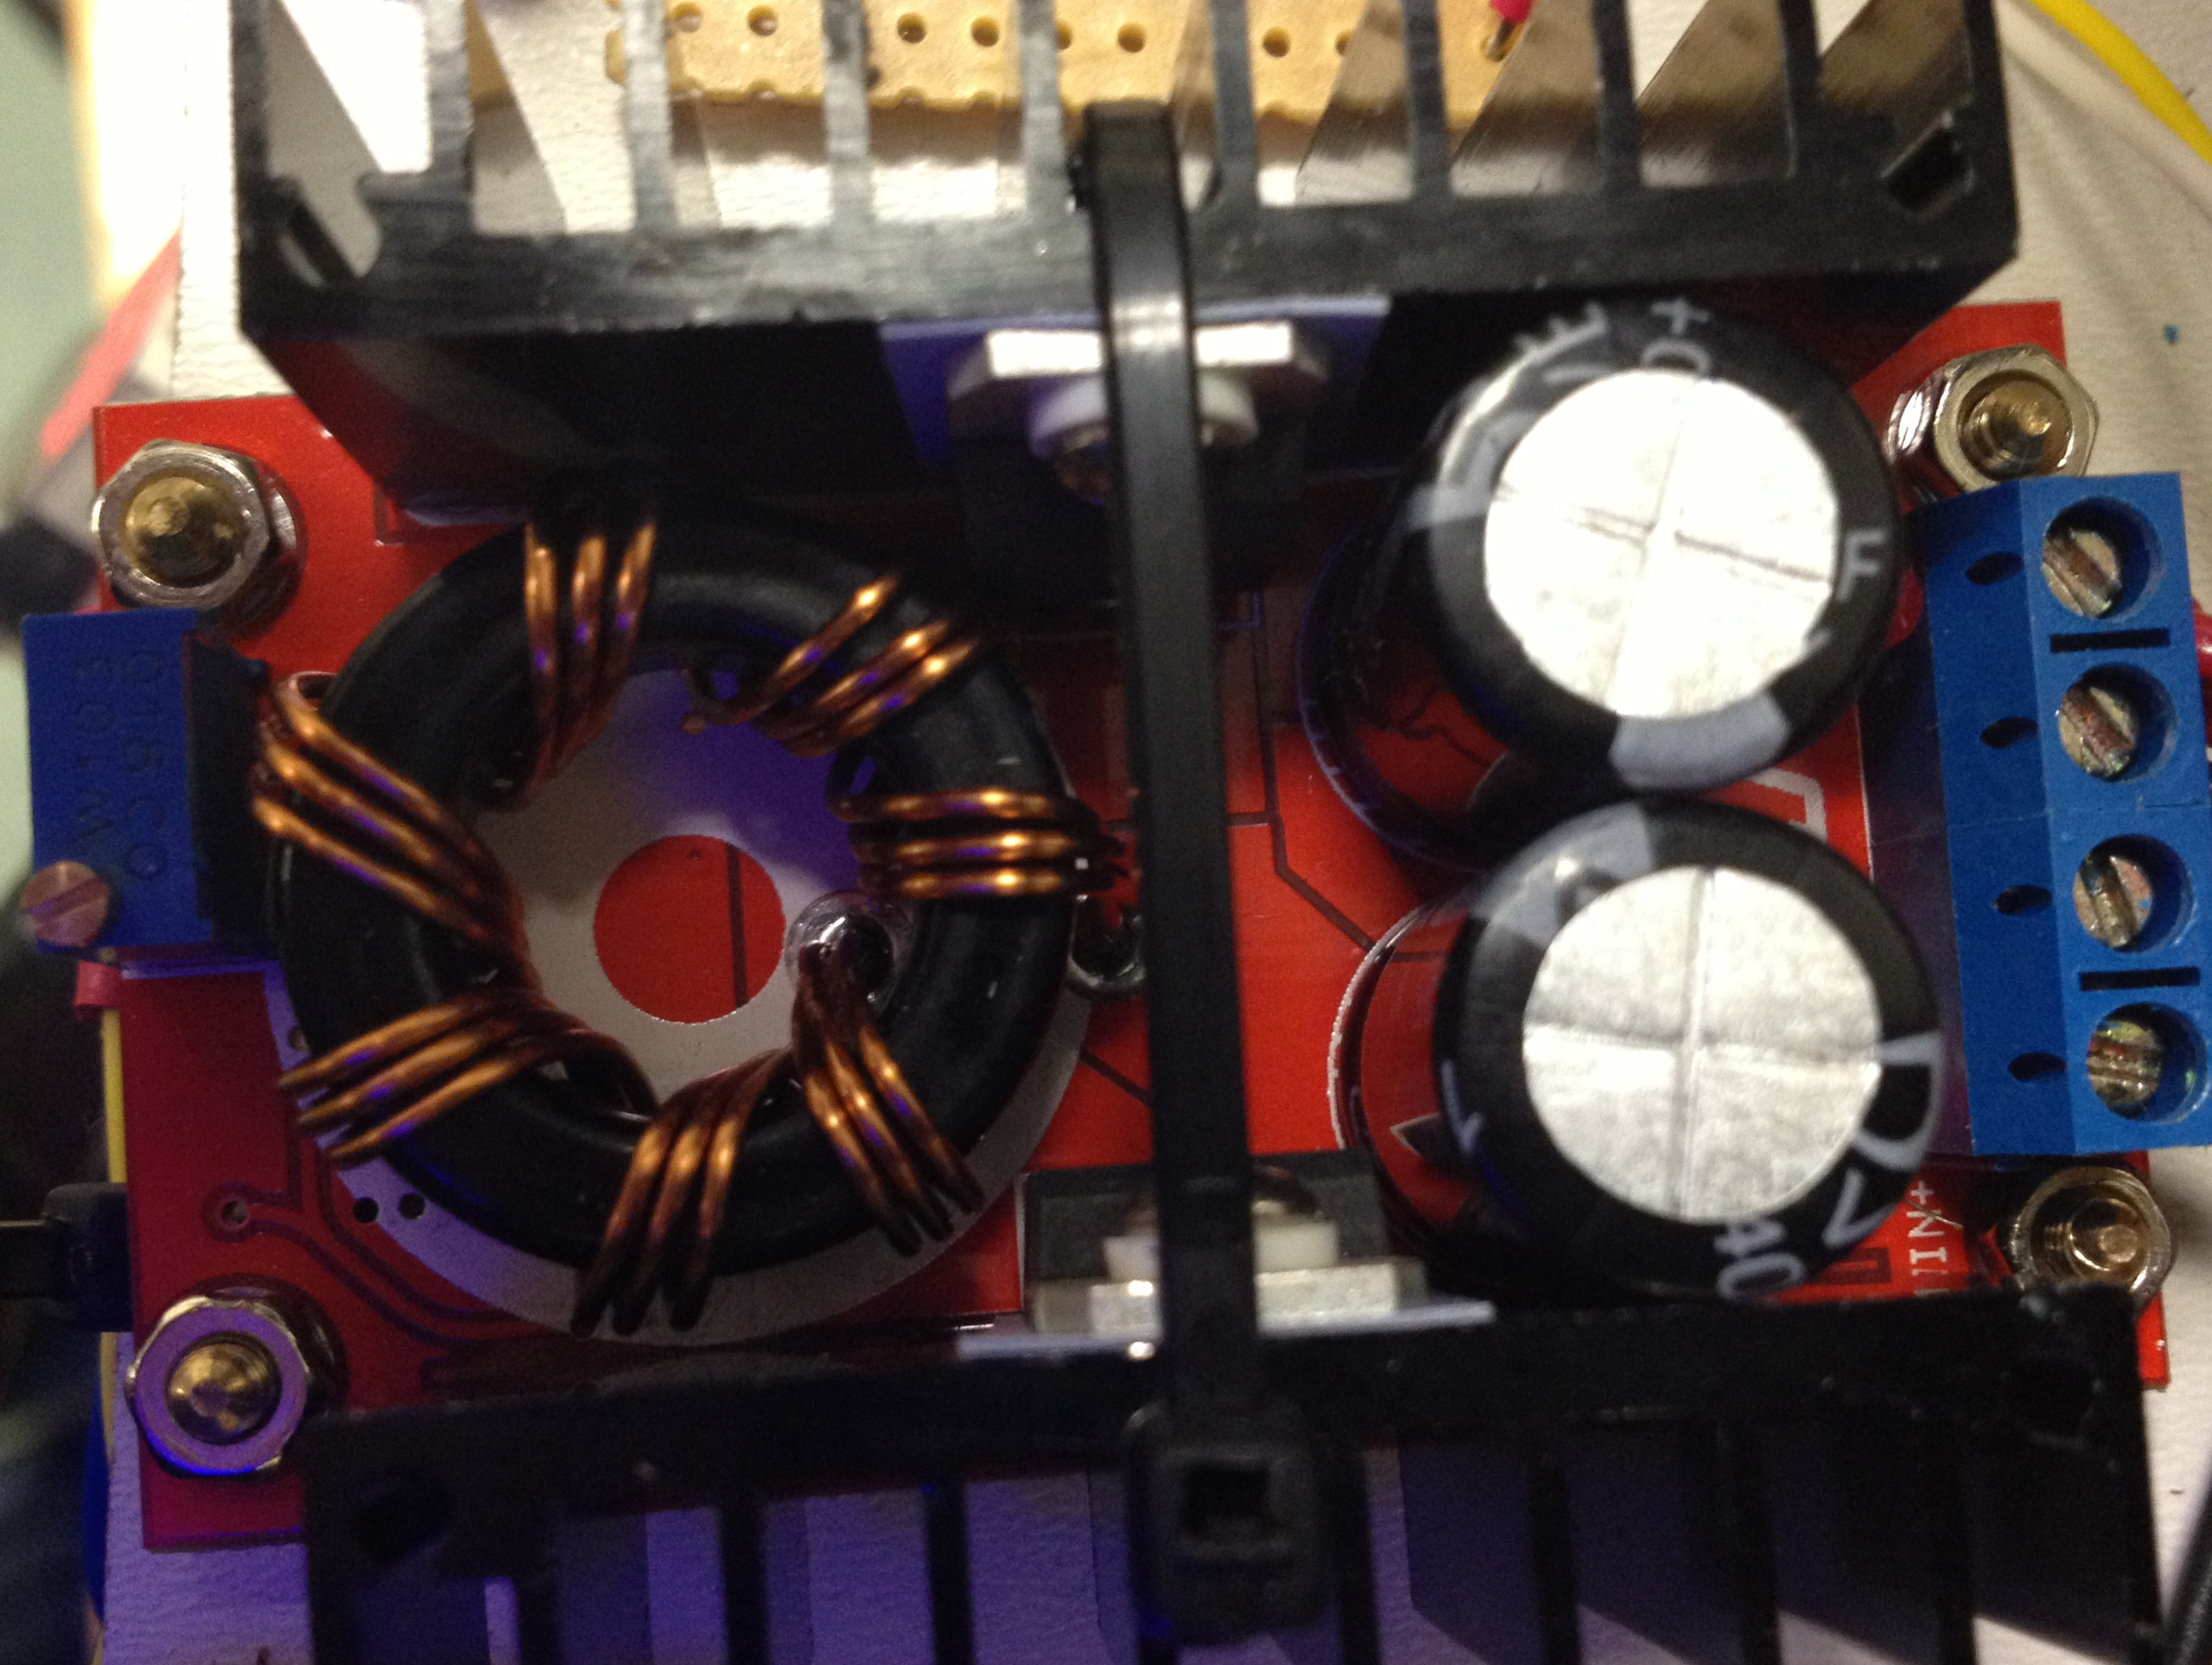
\includegraphics[scale=0.1]{fig/alim_24V_photo.png}
\caption{Figure présentant une photo de l'alimentation 24V pour les périphériques}
\label{fig:alim24Vphoto}
\end{figure}

\begin{figure}[htbp]
\centering
\includegraphics[scale=0.5]{fig/plan_manchester.png}
\caption{Figure présentant les plans du récepteur Manchester}
\label{fig:manchester}
\end{figure}

\begin{figure}[htbp]
\centering
\includegraphics[scale=0.5]{fig/prehenseur.jpg}
\caption{Figure présentant les plans du circuit de commande du préhenseur}
\label{fig:prehenseur}
\end{figure}

\begin{figure}[htbp]
\centering
\includegraphics[scale=0.5]{fig/del_verte.jpg}
\caption{Figure présentant les plans du circuit de commande du préhenseur}
\label{fig:del_verte}
\end{figure}